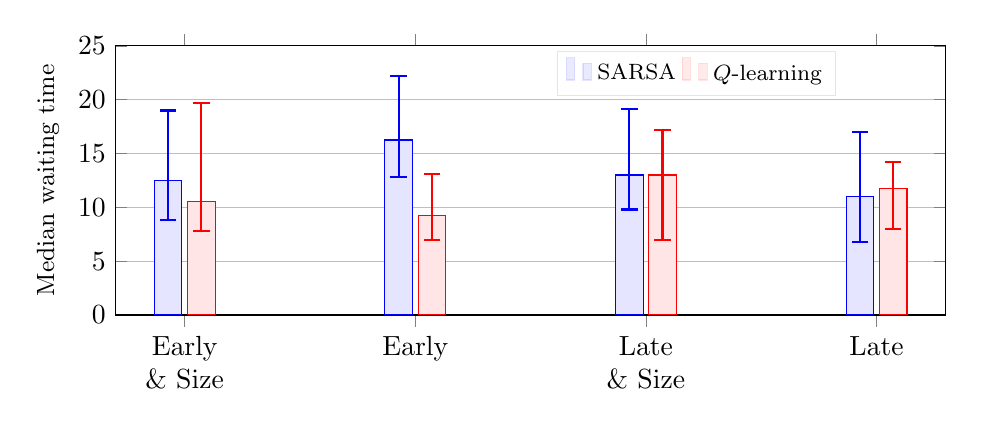
\begin{tikzpicture}

\begin{axis}[
    ybar,
    width = \columnwidth,
    height = 5cm,
    legend style={
        font=\footnotesize,
        fill opacity=0.8,
        draw opacity=0.1,
        text opacity=1,
        at={(0.7,0.98)},
        anchor=north,
        legend columns=-1
    },
    x grid style={white!69.0196078431373!black},
    %xlabel={\small},
    xtick={0, 1, 2, 3},
    xticklabels={
        Early \& Size,
        Early,
        Late \& Size,
        Late
    },
    xticklabel style={text width=50pt, align=center},
    % x tick label style={rotate=45,anchor=east},
    ylabel={\small Median waiting time},
    ymin=0,
    ymax=25,
    ytick={0, 5, 10, 15, 20, 25},
    ylabel near ticks,
    error bars/y dir=both,
    error bars/y explicit=true,
    error bars/error bar style={thick},
    error bars/error mark options={
          rotate=90,
          mark size=3pt,
          thick,
    },
    ymajorgrids,
]

% SARSA
\addplot [
    fill=blue!10!white,
    draw = blue,
    error bars/error mark options/.append={blue}
] table [
    x=x,
    y=y,
    y error minus=y_lower,
    y error plus=y_upper
] {
x    y       y_lower  y_upper
0   12.5    3.7           6.5 
1   16.25    3.45          5.95  
2   13.    3.2           6.1 
3   11.     4.2           6.
};
\addlegendentry{SARSA}

% Q-learning
\addplot [
    fill=red!10!white,
    draw = red,
    error bars/error mark options/.append={red}
] table [
    x=x,
    y=y,
    y error minus=y_lower,
    y error plus=y_upper,
] {
x    y       y_lower  y_upper
0   10.5    2.7      9.2
1    9.25   2.25     3.85
2   13.     6.       4.2
3   11.75   3.75     2.45
};
\addlegendentry{$Q$-learning}


\end{axis}
\end{tikzpicture}

% Sarsa M
%28.   0.  32.5  0. 
%7.2 0.  6.7 0. 
%6.2 0.  6.5 0.2

%QL M
%24.5  0.  31.   0.5
%5.7 0.  7.2 0.5
%8.7 0.  8.  4.7
